\section{Studie av konvektionsparametern}

Finita element har använts för att studera konvektionsparametern. Hastigeterna är alla
satta till noll på randerna med $h=\unit[6,19]{Wm^{-2}K^{-1}}$ vilket motsvrar en helt vindstilla dag.
på de öppna randerna. Husets tak är adiabadiskt
och problemet är studerat under en natt i jämviktsläge (det vill säga en evig natt) med
$T_{ref} = \unit[0]{^\circ C}$ som referenstemperatur och $T_{inne} = \unit[20]{^\circ C}$ inomhus.
Väggens U-värde är satt till $U = \unit[1,19]{Wm^{-2}K^{-1}}$ vilket motsvarar söderväggen på fastigheten på Walleriusgatan. Penaltyparametern är satt til $\lambda = 10^7$.

\begin{figure}
\centering
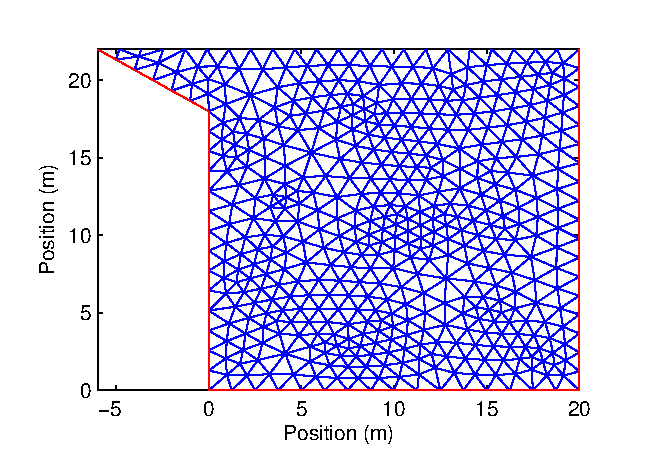
\includegraphics{images/triconvec.eps}
\caption{Definitionsmängd samt triangulering av problemuppställningen för studie av konvektion.}
\end{figure}

Svartkroppsstrålningen approximeras med första ordningens Taylorutveckling och
för varje steg löses det slutgiltiga ekvationssystemet med den
modifierade Newton-Raphson metoden. När systemet har blivit löst beräknas
medeltemperaturen på väggen. Denna används då som gissning och utvecklingspunkt
för ovan nämnda taylorutveckling. Denna process upprepas tills medeltemperaturen
ligger tillräckligt nära gissningen. Således så genomförs en rad Newtonsteg
för att hitta hur mycket som strålar från fastigheten genom svartkroppsstrålning.

Sist beräknas konvektionsparametern genom att vi vet mängden energi som transporteras
genom luften. I jämvikt gäller ekvation \eqref{eq:convectionmethod:balance}.
Här är $Q_v$ energin som flödar genom väggen, $Q_{sk}$ är energin från
svartkroppsstrålning och $Q_k$ är då energin som konvektion transporterar
för att jämvikt skall uppstå.

\begin{equation}
\label{eq:convectionmethod:balance}
Q_v + Q_{sk} = Q_k
\end{equation}

Medeltemperaturen $\bar{T}$ på väggen och referenstemperaturen $T_\infty$ är kända
vilket ger att h-värdet kan beräknas enligt

\begin{align}
Q_k &= h(\bar{T}-T_\infty) \Rightarrow \nonumber \\
h &= \frac{Q_v + Q_{sk}}{\bar{T}-T_\infty}
\end{align}


\begin{figure}[hpbt]
\centering
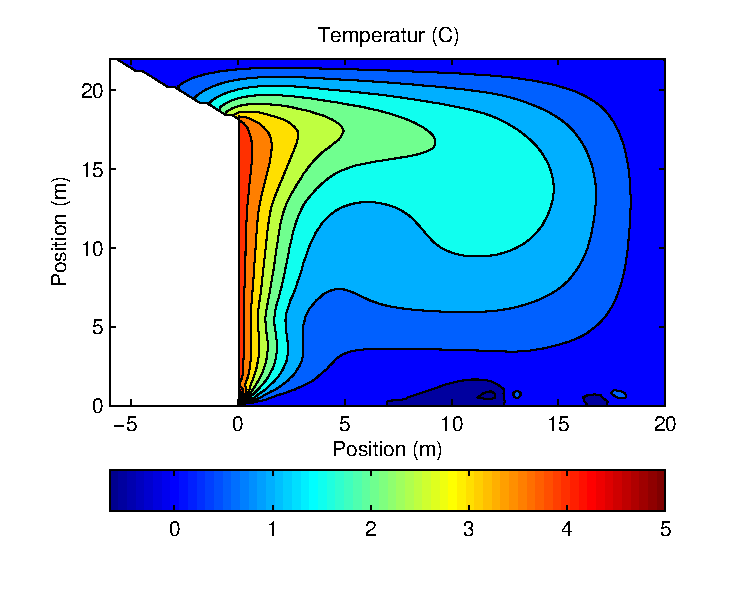
\includegraphics[width=10cm]{images/convectemperature.eps}
\caption{\label{fig:temp_dist}Temperaturfördelningen i $^\circ\mbox{C}$ utanför en vägg, beräknad med finita element av penaltymetoden. Inomh\
ustempertur $\unit[20]{^\circ C}$, utomhustemperatur $\unit[0]{^\circ C}$.}
\end{figure}

% RESULTAT                                                                                                                                    
Denna metod har slutligen verifierasts. Som kan ses i figuren \ref{fig:temp_dist} är luften närmast väggen upp till fem grader
högre än omgivningen. När det blåser försvinner den här temperaturskillnaden. Detta
visar tydligt hur viktigt det är att inte bara reglera efter utomhustemperaturen.
Här finns dock anomala temperaturer vid nedre randen. Detta tyder på problem med
metodiken.
%%%%%%%%%%%%%%%%%%%%%%%%%%%%%%%%%%%%%%%%%%%%                                                                                                  
Även hastighetsfältet för temperaturens flöde, då det är vindstilla, har beräknats med finita element metoden
applicerad på penaltymetoden. Detta kan ses i figur \ref{fig:velocityfield} där också
beloppet av hastighetsfältet syns och det kan noteras att hastigheterna orimligt små.

\begin{figure}[hpbt]
\begin{center}
\subfloat[Hastighetsfält]{
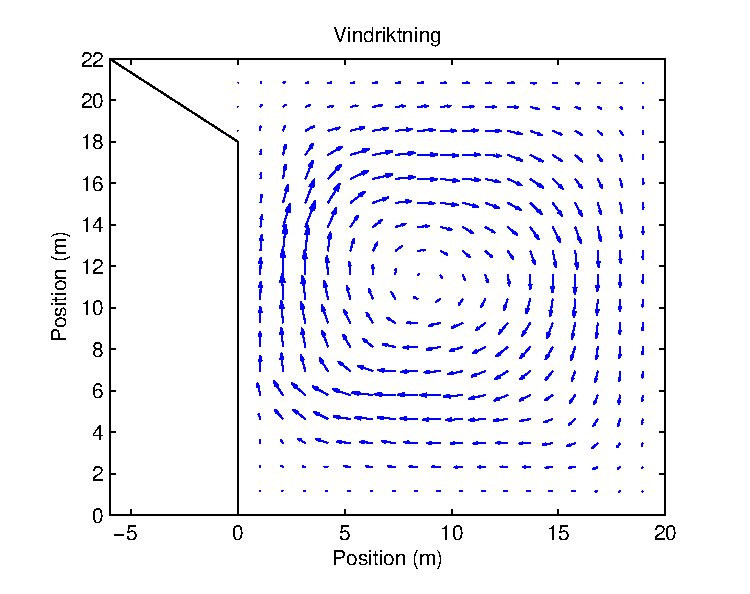
\includegraphics[scale=0.5]{images/convecquiver.eps}
}
\subfloat[Beloppet av hastigheten]{
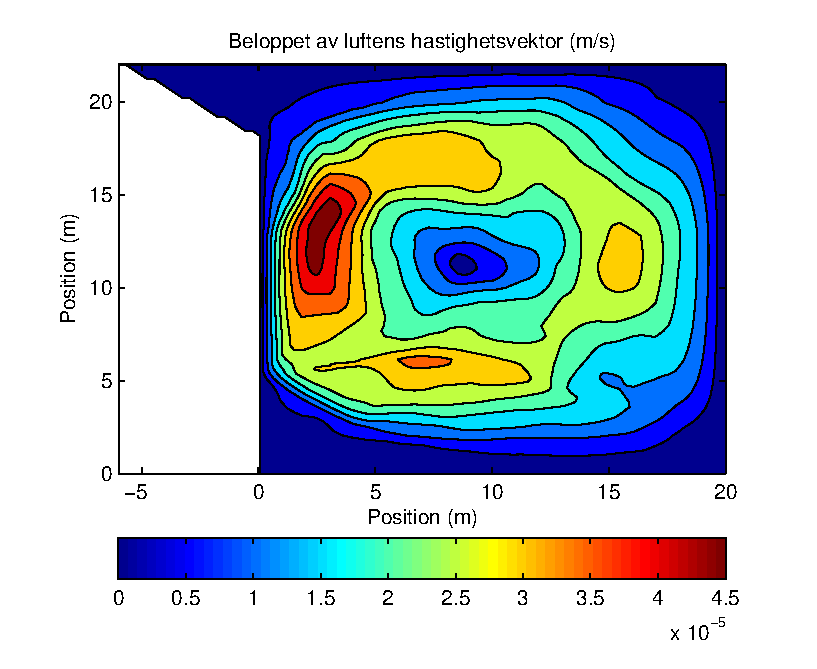
\includegraphics[scale=0.5]{images/convecspeed.eps}
}
\caption{\label{fig:velocityfield} Hur luften vid husväggen flödar vid en temperaturskillnad.}
\end{center}
\end{figure}

Då vi i sedan utifrån detta beräknar konvektionsparametern blir den därför väldigt liten,
se figur \ref{fig:konv_param}. Tyvärr verkade det inte som att metodiken som användes
för att framställa ovanstående data fungerade tillräckligt bra för att med någon
noggrannhet studera fenomenet konvektion.  Vi menar dock att formen på hastighetsflödet intill marken och väggen
kan anses vara av rätt karaktär och visar på hur luften rör sig vid husväggen. Dock kan randerna mot
luft påverka då det ej var tillåtet för luften att passera de
kanterna. Detta kan också vara en felkälla till den absurt låga konvektionsparametern.

\begin{figure}[hpbt]
\centering
\subfloat[\label{fig:h_reftemp}Konvektionskoefficienten h mot referenstemperaturen]{
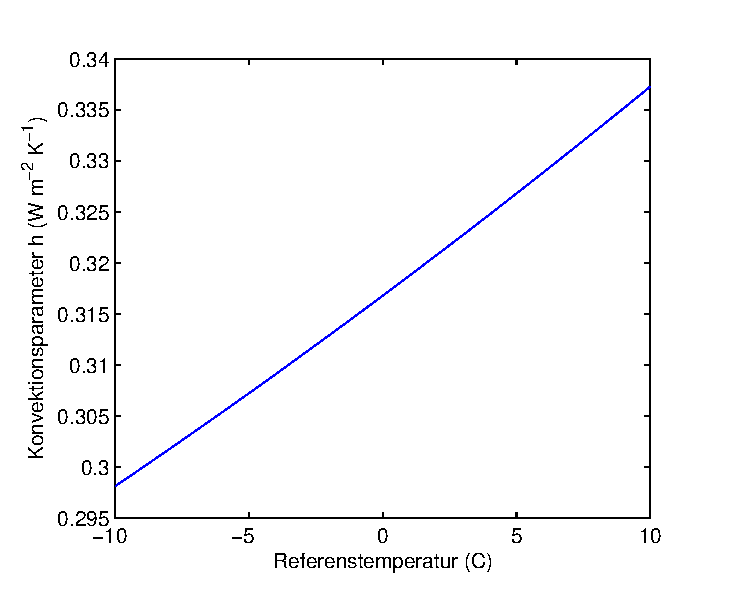
\includegraphics[scale=0.5]{images/convech.eps}
}
\subfloat[\label{fig:h_penalty}Konvektionskoefficienten h mot penaltyparametern]{
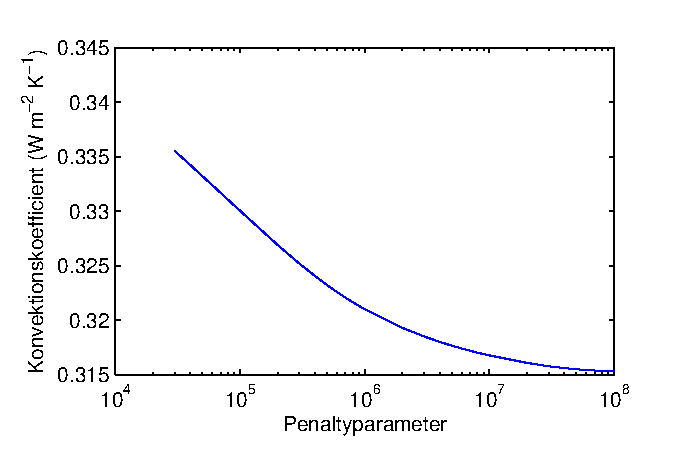
\includegraphics[scale=0.5]{images/convecpenalty.eps}
}\vspace{1cm}

\subfloat[\label{fig:h_volexp}Konvektionskoefficienten h mot den volymetriska expansionskoefficienten.]{
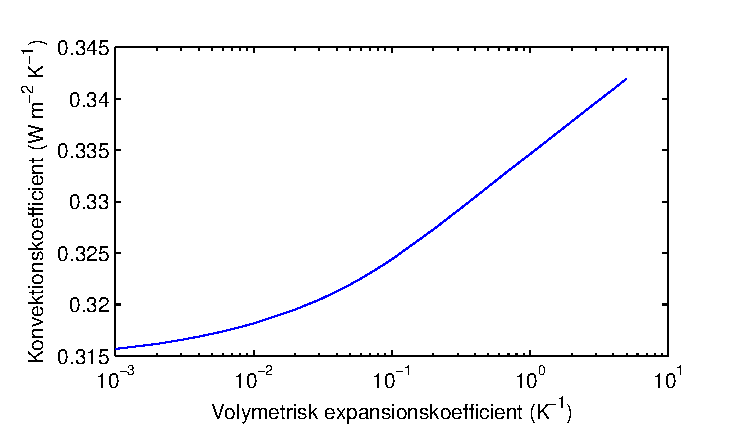
\includegraphics[scale=0.5]{images/convecbeta.eps}
}

\caption{\label{fig:konv_param}Stabilitetsberäkningar av konvektionskoefficienten h mot några
parametrar och naturkonstanter i finita elementsimuleringen av Navier-Stokes ekvationer.
Inomhustemperaturen är satt till konstanta $\unit[20]{^\circ C}$ med en vägg vars U-värde är
$\unit[1,19]{ Wm^{-2}K^{-1}}$. Detta skall motsvara söderväggen på fastigheten som detta arbete behandlar.}

\end{figure}

% RESULTAT                                                                                                                                    
I figur \ref{fig:h_reftemp} har finita elementmodellens beteende studerats vid variation på några essentiella storheter i modellen.
Först har penaltyparametern varierats i figur \ref{fig:h_penalty} och här kan det ses att modellens beteende förändras inte nämnvärt
beroende på val av parameter när denna börjar vara i storleksordningen $\lambda = 10^7$. Det linjära förhållandet mellan
konvektionskoefficienten och temperaturdifferansen är intressant men saknar stöd i litteraturen då den rimligtvis borde vara
konstant eller nästan konstant. Slutligen varieras den volymetriska expansionskoefficienten
i figur \ref{fig:h_volexp}. Det är denna storhet
som gör att luften stiger när den blir varm och av denna anledning fenomenet fri konvektion uppstår. Konvektionskoefficienten
ser ut att öka mer än logaritmiskt men däremot ej så snabbt. Anledningen till att denna parameter varierades var för
att se hur stor den parametern skulle behöva bli innan konvektionen började få samma energitransporterande egenskaper
som den borde ha. Som kan ses så kommer inte modellen ens i närheten vid en väldigt stort vald volymetrisk expansionskoefficient.

Slutligen kan vi bara konstatera att det ej gick att använda denna metod för att stude\
ra konvektionsparametern $h$. Litteraturen
som har använts som grund till detta har använt sig av Streamline-Upwind/Petrov-Galerk\
in (SUPG). \cite{heinrich88}\cite{roy05} Ovanstående metod är dock
Standard Galerkin med linjära triangulära element. Det är känt att Standard Galerkin kan leda till korsvindsproblem oc\
h lösningar som ej är
exakta och stabila.\cite{segal2011}
En misstanke är att det är detta problem vi ser trots att detta ej verifieras genom at\
t titta på hastighetsfältet. Andra
möjliga orsaker kan vara randvillkor, för liten vald definitionsmängd eller något fel \
i den matematiska beskrivningen alternativt
matlab-implementeringen.
